\documentclass[runningheads]{llncs}

\usepackage{booktabs}
\usepackage{amsmath}
\usepackage{amssymb}
\usepackage{graphicx}
\usepackage{xcolor}
\usepackage{enumitem}
\usepackage{placeins}
\usepackage{tabularx}
\setlist{nosep,leftmargin=*}
\providecommand{\texorpdfstring}[2]{#1}

\newcommand{\1}{\mathbf{1}}
\newcommand{\sigmoid}{\operatorname{logit}^{-1}}
\newcommand{\E}{\mathbb{E}}
\newcommand{\Var}{\operatorname{Var}}
\newcommand{\DeltaCV}{\Delta_{\text{CV}}}

\begin{document}

\title{The Autocorrelation Mirage: Dependence-Aware Evaluation for Panel-Expanded Event Forecasting}
\titlerunning{Dependence-Aware Evaluation for Panel-Expanded Forecasting}

\author{Behnaz Moradi-Jamei\inst{1}\thanks{Corresponding author: \texttt{moradibx@jmu.edu}.} \and Ali Tavasoli\inst{1}}
\authorrunning{B. Moradi-Jamei and A. Tavasoli}
\institute{Department of Mathematics and Statistics, James Madison University, Harrisonburg, VA 22807, USA\\
\email{\{moradibx,hqyq4k\}@jmu.edu}}

\maketitle

\begin{abstract}
Panel expansion can turn a small collection of independent episodes into many dependent rows. When row-wise cross-validation places rows from an episode in both training and test folds, it answers an interpolation question even when deployment requires generalization to unseen episodes. We call the resulting mechanism \emph{episode memorization}; latent episode heterogeneity and shared event-time structure, not autocorrelation alone, drive the effect. In a controlled simulation with strictly causal features, row-wise five-fold cross-validation raises boosted-tree AUROC from 0.552 to 0.835 ($\DeltaCV=0.283$, paired 95\% CI [0.246, 0.320]). A higher-signal configuration has nontrivial grouped AUROC (0.723), yet retains a 0.199 gap (95\% CI [0.170, 0.229]). A 10-replicate-per-cell grid finds larger gaps for tree ensembles than logistic regression. A separate drift-based DGP (30 replicates per model) finds a smaller normalization-leakage effect; it is distinguishable from zero only for random forests. We propose reporting grouped and row-wise estimates, fold-local preprocessing, and $\DeltaCV$ as a practical diagnostic. All empirical evidence is simulation-based.

\keywords{pseudoreplication, cross-validation, panel data, event forecasting, episode memorization}
\end{abstract}

\section{Introduction}

Consider a hospital forecasting deterioration within two weeks from daily vital signs for only 30 patients. Expanding stays into daily rows yields hundreds of records, as in maintenance and conflict forecasting~\cite{hegre2019,muchlinski2016}, but not hundreds of independent trajectories. If deployment is for an unseen patient, row-wise K-fold can place that patient's rows in both training and test sets and answer an interpolation question instead.

We call this \textbf{episode memorization}: a flexible model exploits latent episode effects, shared event-time structure, or trajectories represented on both sides of a split rather than transferable signal. It differs from \emph{explicit leakage}, which encodes unavailable future information (e.g., $T_e-t$), and \emph{preprocessing leakage}, which admits test or future observations into a transform. Pseudoreplication is instead an evaluation-unit mismatch and can occur with strictly causal features.

We quantify the mismatch, test it with nontrivial transferable signal, isolate its mechanisms, and contrast it with preprocessing leakage. Our practical diagnostic is $\DeltaCV$, the row-wise minus grouped AUROC. The paper reviews related validation work, specifies the DGP and protocols, presents results, and closes with a deployment-focused checklist. Evidence is simulation-based.

\section{Related Work}\label{sec:related}

Grouped, blocked, and subject-wise validation align the held-out unit with structured deployment~\cite{roberts2017,prado2018}; record-wise evaluation can overstate subject-wise performance in clinical and wearable ML~\cite{saeb2017,vabalas2019}. Hurlbert~\cite{hurlbert1984} termed treating non-independent observations as replicates \emph{pseudoreplication}. Leakage taxonomies distinguish information unavailable at prediction time~\cite{kaufman2012,kapoor2023}, while temporal and panel-forecasting studies show that a splitter can overturn conclusions~\cite{cranmer2017,neunhoeffer2019}. We isolate evaluation-unit mismatch alongside explicit and preprocessing leakage in one controlled event-time DGP.

\section{Theoretical Framework}\label{sec:theory}

Consider $E$ episodes indexed by $e$. Each has time $t \in \{0,\ldots,T_{\max}\}$, administrative censoring time $C_e$, observed-event indicator $\delta_e := \1\{\text{event observed by } C_e\}$, features $X_{e,t} \in \mathbb{R}^p$, and static attributes $\alpha_e$. When $\delta_e = 1$, let $T_e$ denote the observed event time. For horizon $H$, eligible rows are
\[
\mathcal{T}_e(H)
:=
\{t : \delta_e = 1,\ t < T_e\}
\cup
\{t : \delta_e = 0,\ t + H \leq C_e\}.
\]
The binary target is
\[
Y_{e,t}(H)
:=
\begin{cases}
\1\{T_e \leq t + H\}, & \delta_e = 1, \\
0, & \delta_e = 0 \text{ and } t + H \leq C_e.
\end{cases}
\]
Late censored rows with $t + H > C_e$ are excluded from the supervised evaluation set rather than labeled heuristically.

Let $\mathcal{F}_{e,t^-} := \sigma(\{X_{e,s} : s < t\} \cup \{\alpha_e\} \cup \mathcal{E}_{<t})$ denote information strictly before $t$.

\begin{definition}[Predictable Feature]
Feature $X_{e,t}$ is \emph{predictable} if it is $\mathcal{F}_{e,t^-}$-measurable, that is, determined by information available before $t$.
\end{definition}

This extends Kaufman et al.'s~\cite{kaufman2012} learn-predict separation to filtrations. Violations need not be explicit: global statistics computed over $\{X_{e,s} : s \leq T_e\}$ implicitly depend on $T_e$.

\begin{definition}[Explicit Leakage]
An observation exhibits \emph{explicit leakage} if a feature is not predictable because it is a direct function of future outcome information such as $T_e - t$.
\end{definition}

\begin{definition}[Normalization Leakage]
\emph{Normalization leakage} occurs when test-fold statistics, future within-episode values, or full-trajectory episode summaries enter transformed inputs even though they would be unavailable at prediction time.
\end{definition}

\begin{definition}[Pseudoreplication]
\emph{Pseudoreplication} occurs when the evaluation split places observations from the same episode in both training and test folds, violating the independence assumptions underlying row-wise validation even if all features are predictable.
\end{definition}

The deployment target for unseen episodes is the episode-level risk
\[
R_{\mathrm{episode}}(f)
=
\E_{e^\star}
\left[
\frac{1}{|\mathcal{T}_{e^\star}|}
\sum_{t\in\mathcal{T}_{e^\star}}
\ell\{f(X_{e^\star,t}),Y_{e^\star,t}\}
\right],
\]
where $e^\star$ is not represented in the training episodes. Episode-grouped validation estimates this target by holding out complete episodes. Row-wise validation instead estimates a conditional interpolation risk closer to
\[
R_{\mathrm{row}}(f)
=
\E
\left[
\ell\{f(X_{e,t}),Y_{e,t}\}
\;\middle|\;
e\in\mathcal{E}_{\mathrm{train}}
\right],
\]
because test rows may share latent episode effects, trajectory structure, and event time with training rows. Thus the issue is not dependence alone; it is a mismatch between the generalization unit implied by deployment and the unit used by validation.

\begin{remark}[Explicit leakage can make ranking nearly perfect]\label{thm:leakage}
Suppose both classes have positive probability and the leaked score has the form $S_{e,t} = f(T_e - t) + \epsilon_{e,t}$, where $f$ is strictly monotone on the support relevant for $Y_{e,t}(H)$ and the learned scoring rule uses the sign convention that smaller time-to-event implies higher risk. Restricting attention to eligible rows from episodes with observed event times (censored no-event rows can be treated as having $T_e - t = \infty$), $Y_{e,t}(H)=1$ iff $T_e - t \in (0,H]$, so a strictly monotone transform of $T_e - t$ induces the same ordering as the raw time-to-event. If $\Var(\epsilon_{e,t}) = \sigma^2$, then as $\sigma^2 \to 0$ the leaked score preserves that ordering almost surely and $\mathrm{AUC} \to 1$. We record this as a sanity check rather than a substantive result: it confirms that a feature built directly from the outcome-defining quantity $T_e - t$ is exactly the kind of explicit leakage that Definition~2 rules out, and it calibrates the explicit-leak condition in Table~\ref{tab:sim} as a near-worst-case comparator rather than a typical one.
\end{remark}

\section{Implicit Violations in Standard Pipelines}\label{sec:implicit}

Explicit leakage exposes post-$t$ outcome information; preprocessing leakage uses test-fold or future within-episode information; pseudoreplication is an evaluation-unit mismatch that splits an episode across folds. Full-trajectory episode means, episode-wise z-scores, imputation, and centered windows can leak future values; transformations must be fit in each training fold.

\section{Episode Memorization Under Row-Wise Cross-Validation}\label{sec:pseudo}

Even with leak-free features, row-wise K-fold can inflate performance when the target is generalization to unseen episodes. This is pseudoreplication in the sense of Hurlbert~\cite{hurlbert1984}: rows from one episode are not independent replicates. They share episode effects $\alpha_e$, correlated features, and a common event history. If some rows appear in training, a flexible model can use that information to predict other rows from the same episode. Grouped validation removes this shortcut. As a descriptive design-effect approximation, if each episode contributes approximately $m$ rows and the average within-episode pairwise correlation is $\bar{\rho}$, then
\[
n_{\text{eff}} \approx \frac{n}{1 + (m-1)\bar{\rho}}.
\]
This approximation is not used for inference; it is reported only to highlight that panel expansion can substantially overstate the amount of independent evidence.

A minimal example makes the mechanism concrete. Suppose episodes A, B, and C each contribute two daily rows. A random two-fold split may train on $\{A_1,B_1,C_2\}$ and test on $\{A_2,B_2,C_1\}$; every test row now has a sibling row from the same episode in training. A grouped split instead trains on $\{A_1,A_2,B_1,B_2\}$ and tests on $\{C_1,C_2\}$, forcing prediction to transfer across episodes rather than match within them.

For $n=600$, $m \approx 20$, and $\bar{\rho} \approx 0.5$, this approximation gives $n_{\text{eff}} \approx 55$---a 10$\times$ reduction. But the inflation from episode memorization is \textit{not} merely a sample-size effect: in the empirical benchmark below, row-wise CV still achieves AUC above 0.8 despite the small effective sample size.

This suggests an empirical expectation that, once within-episode dependence is present, row-wise CV will exceed grouped CV more strongly for higher-capacity models. Section~\ref{sec:empirical} tests that expectation directly over a compact grid of dependence levels, episode counts, dimensionalities, and model families.

\begin{proposition}[Sibling overlap under shuffled row-wise K-fold]\label{prop:overlap}
Consider an episode with $m_e$ eligible rows assigned independently to one of $K$ folds. Condition on one row being placed in the test fold. Then the probability that at least one of its $m_e-1$ sibling rows appears in the training folds is
\[
\Pr(\text{sibling overlap}) = 1 - K^{-(m_e-1)},
\]
and the expected number of same-episode training siblings is
\[
\mathbb{E}[N_{\text{sibling in train}}] = (m_e-1)\frac{K-1}{K}.
\]
\end{proposition}

\textit{Proof sketch.} Condition on the test row being assigned to fold $k$. Its siblings avoid the training set only if they also fall in fold $k$, which under independent fold assignment occurs with probability $K^{-(m_e-1)}$. The complement gives the overlap probability, and linearity of expectation yields the expected sibling count. The exact probability differs slightly for deterministic balanced K-Fold, but the approximation captures the usual shuffled row-wise setting. \qed

\section{Empirical Validation}\label{sec:empirical}

We generate $E=30$ episodes with $\alpha_e \sim \mathcal{N}(0,0.5)$, $Z_{e,t}=0.7Z_{e,t-1}+\epsilon_t$, and $h_{e,t}=\sigmoid(-3+\alpha_e+0.15Z_{e,t})$. Features use only $Z_{e,<t}$. Episodes are administratively censored at $C_e=T_{\max}=60$. Observed-event rows are eligible before $T_e$ and receive $Y_{e,t}(14)=\1\{T_e\leq t+14\}$; censored rows are eligible only when their full horizon is observed. Late censored rows are excluded. Across 10 seeds, the filtered panel has about 587 rows, mean episode length 19.6, episode-event frequency 0.91, and positive-row prevalence 0.48.

The five base features are causal transformations of $Z_{e,<t}$; the robustness grid adds nuisance features to reach $p\in\{20,100\}$. The main model is histogram gradient boosting (100 iterations, depth 4, learning rate 0.1). Main grouped and row-wise analyses use five folds; the robustness grid uses three. Temporal blocking estimates the separate target of forecasting later rows from known episodes.

Each replicate yields pooled out-of-fold AUROC and Brier scores; we also calculate episode-weighted diagnostics. Standardization is fit within each training fold except in deliberate leakage conditions. Matched seeds make the split comparisons paired, and 95\% intervals use matched replicate differences, $\bar d \pm t_{0.975,n-1}s_d/\sqrt n$. The main, higher-signal, and drift analyses use 30 replicates; the robustness grid uses 10 per cell.

\begin{table}[t]
\centering
\caption{Simulation results over 30 paired replicates. Also shown is a grouped training-fold prevalence predictor; the temporal-blocked within-episode baseline is reported in text because it targets a different estimand.}\label{tab:sim}
\scriptsize
\begin{tabular}{@{}p{3.2cm}cccc@{}}
\toprule
Condition & AUC & Brier & $\Delta$AUC vs.\ baseline & 95\% paired CI \\
\midrule
Leak-Free + Grouped CV & 0.552 $\pm$ 0.101 & 0.330 $\pm$ 0.048 & baseline & -- \\
Training-Fold Prev. + Grouped CV & 0.430 $\pm$ 0.025 & 0.245 $\pm$ 0.009 & -0.122 & [-0.159, -0.086] \\
Leak-Free + Row-wise KFold & \textbf{0.835 $\pm$ 0.040} & 0.162 $\pm$ 0.023 & \textbf{+0.283} & [0.246, 0.320] \\
Global Norm. + Grouped CV & 0.552 $\pm$ 0.101 & 0.330 $\pm$ 0.048 & +0.000$^\dagger$ & [0.000, 0.000] \\
Explicit Leak + Grouped CV & 0.813 $\pm$ 0.042 & 0.198 $\pm$ 0.041 & +0.261 & [0.236, 0.286] \\
\bottomrule
\multicolumn{5}{l}{\footnotesize $^\dagger$See text for interpretation.}
\end{tabular}
\end{table}

Table~\ref{tab:sim} gives the central result: row-wise KFold yields AUROC 0.835 from strictly causal features versus 0.552 grouped ($\DeltaCV=0.283$, 95\% CI [0.246, 0.320]). Explicit $T_e-t$ leakage raises grouped AUROC by 0.261 [0.236, 0.286]. For future rows of known episodes, temporal-blocked validation yields AUROC 0.917; it is not an unseen-episode estimate because same-episode history remains in training. Global scaling has no effect in this stationary DGP; the drift experiment provides the preprocessing-leakage example.

\begin{table}[t]
\centering
\caption{$\DeltaCV$ by episode count $E$ instead of dependence, averaged over $\rho$ and $p$ (10 replicates per cell).}\label{tab:grid-episodes}
\small
\begin{tabular}{@{}lccc@{}}
\toprule
Model family & $E = 20$ & $E = 50$ & $E = 100$ \\
\midrule
Logistic regression & 0.047 & 0.029 & 0.012 \\
Random forest & 0.177 & 0.150 & 0.117 \\
Boosted trees & 0.203 & 0.205 & 0.190 \\
\bottomrule
\end{tabular}
\end{table}

\subsection{Does the Gap Survive a Genuinely Non-Trivial Grouped Baseline?}\label{sec:highsignal}

The grouped AUROC in Table~\ref{tab:sim} is 0.552. We therefore considered a higher-signal configuration. Increasing the state-to-hazard coefficient $\beta$ across 0.15--1.3 left grouped AUROC near chance (0.537--0.580 over 10 replicates per setting), because the episode-specific trajectory does not transfer to held-out episodes. We instead raise the standard deviation of $\alpha_e$ from 0.5 to 1.5, holding other parameters fixed. The static feature $X_5$ measures this episode-level risk component with small noise, so it can transfer from training episodes to a held-out episode. Over 30 paired replicates, grouped AUROC is 0.723 $\pm$ 0.099 and row-wise AUROC is 0.922 $\pm$ 0.039. The gap is 0.199 [0.170, 0.229] (Table~\ref{tab:highsignal}).

\begin{table}[t]
\centering
\caption{Raising the episode-effect standard deviation from 0.5 to 1.5 (30 paired replicates each, DGP otherwise identical) more than doubles grouped-CV AUC while the row-wise gap remains large.}\label{tab:highsignal}
\small
\begin{tabular}{@{}lccc@{}}
\toprule
Configuration & Grouped AUC & Row-wise AUC & $\DeltaCV$ (95\% CI) \\
\midrule
Baseline (episode-effect sd $=0.5$) & 0.552 $\pm$ 0.101 & 0.835 $\pm$ 0.040 & 0.283 [0.246, 0.320] \\
Higher signal (episode-effect sd $=1.5$) & 0.723 $\pm$ 0.099 & 0.922 $\pm$ 0.039 & 0.199 [0.170, 0.229] \\
\bottomrule
\end{tabular}
\end{table}

Across the 81 robustness cells (10 paired replicates each), tree ensembles show larger gaps than logistic regression; gaps increase with dependence and remain with nuisance dimensions up to $p=100$. Table~\ref{tab:grid-episodes} shows the episode-count trend: gaps generally fall as $E$ grows, but remain substantial for tree ensembles at $E=100$.

The nonzero gap at $\rho=0$ shows that the effect is not driven by autocorrelation alone. Episode-level latent heterogeneity and shared event-time structure can already create row-wise optimism; increasing autocorrelation strengthens the same evaluation-unit mismatch.

For normalization leakage, a second DGP adds the drift term $\text{drift\_strength}(t/T_{\max})$ to $Z_{e,t}$, with drift strength 1.0; other parameters match the main benchmark. Full-trajectory episode normalization then uses future within-episode values.

Over 30 paired replicates per model, grouped AUROC increases by 0.045 for logistic regression (95\% CI [--0.010, 0.100]), 0.063 for random forests ([0.029, 0.096]), and 0.034 for boosted trees ([--0.010, 0.077]). Global standardization has no measurable effect. Only the random-forest interval excludes zero.

The normalization effect is smaller than the row-splitting effect and requires more replication to estimate precisely. Earlier lightly replicated pilot estimates were noisier and are not reported.

Figure~\ref{fig:robustness_drift} shows larger $\DeltaCV$ values for tree-based learners and higher drift-DGP AUROC under full-trajectory normalization, most clearly for random forests.

\begin{figure}[!htbp]
\centering
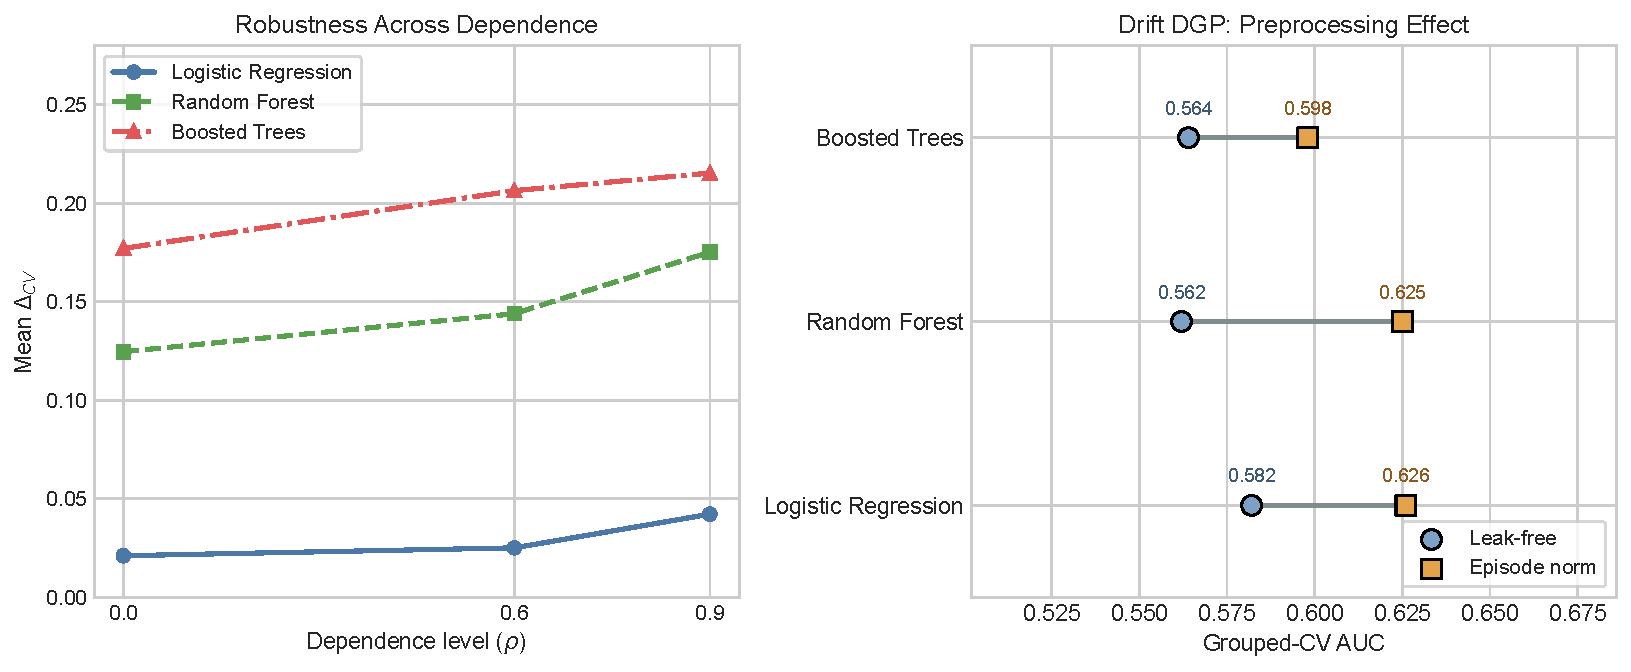
\includegraphics[width=0.94\textwidth]{robustness_drift_companion.pdf}
\caption{Companion diagnostics for the strengthening experiments. Left: mean $\DeltaCV$ versus dependence after averaging over $E$ and $p$ for each model family. Right: grouped-CV AUC in the drift DGP under leak-free inputs and full-trajectory episode normalization; global standardization overlaps the leak-free baseline and is omitted for clarity.}
\label{fig:robustness_drift}
\end{figure}

\paragraph{Mechanism isolation.} Table~\ref{tab:ablation} uses a matched-prevalence negative control. The fingerprint-off condition removes $X_5$ and all episode-constant random features. The shared-event-time-off condition uses fixed-length episodes and independent row outcomes, so it is not an event-forecasting model. With both factors off, the gap is -0.001 [--0.008, 0.006]. Shared event-time labeling alone produces 0.038 [0.028, 0.048], and the fingerprint alone produces 0.006 [--0.001, 0.014]. Both together recover 0.283 [0.246, 0.320]. Thus, neither isolated factor reproduces the headline effect; their combination does in this DGP.

\begin{table}[t]
\centering
\caption{Mechanism isolation (30 paired replicates/cell). The event-time-off cells are fixed-length, independent-row negative controls.}\label{tab:ablation}
\scriptsize
% Generated; do not edit manually.
\begin{tabular}{llccc}
\toprule
Fingerprint & Shared event time & Grouped & Row-wise & $\Delta_{\rm CV}$ (95\% CI) \\
\midrule
off & off & 0.505 & 0.504 & -0.001 [-0.008, 0.006] \\
off & on & 0.498 & 0.535 & 0.038 [0.028, 0.048] \\
on & off & 0.492 & 0.498 & 0.006 [-0.001, 0.014] \\
on & on & 0.552 & 0.835 & 0.283 [0.246, 0.320] \\
\bottomrule
\end{tabular}

\end{table}

\FloatBarrier

\section{\texorpdfstring{The $\Delta_{\mathrm{CV}}$ Diagnostic and Dependence-Aware Evaluation Protocol}{The DeltaCV Diagnostic and Dependence-Aware Evaluation Protocol}}
\label{sec:delta-cv-protocol}

We propose a simple diagnostic for split sensitivity under panel expansion:

\begin{definition}[$\DeltaCV$ diagnostic]
Let $\widehat{\mathrm{AUC}}_{\mathrm{row}}$ denote the pooled out-of-fold AUROC under row-wise KFold and let $\widehat{\mathrm{AUC}}_{\mathrm{group}}$ denote the pooled out-of-fold AUROC under episode-grouped KFold. We define
\[
\Delta_{\mathrm{CV}}
=
\widehat{\mathrm{AUC}}_{\mathrm{row}}
-
\widehat{\mathrm{AUC}}_{\mathrm{group}}.
\]
Large positive values indicate split sensitivity: the model performs better when test rows are allowed to share episodes with training rows than when entire episodes are held out.
\end{definition}

In our main benchmark, $\DeltaCV = 0.283$. In the robustness grid, logistic regression usually stays near zero, whereas random forests and boosted trees remain well above 0.10 on average and grow with $\rho$. That pattern makes values around 0.05 a useful warning heuristic in our setting, but we do not claim a universal decision threshold. The relevant magnitude will depend on the domain, target definition, dependence strength, and model family. This metric requires no additional data collection---only re-running evaluation with episode-grouped validation instead of row-wise \texttt{KFold}.

\textbf{Dependence-Aware Evaluation Protocol:} (1)~\textit{Preprocessing:} fit transformations on training folds only; use forward-fill imputation and trailing windows. (2)~\textit{Evaluation:} use grouped splitting with \texttt{groups=episode\_id}; never split episodes across folds. (3)~\textit{Reporting:} report $\DeltaCV$ and $n_{\text{eff}}$ alongside AUC.

\textbf{Minimal algorithm:} (1)~construct labels only for rows whose $H$-step outcome is observed; (2)~choose the split protocol that matches the deployment target; (3)~fit preprocessing on each training fold only; (4)~fit the model and predict held-out rows; (5)~aggregate pooled and episode-weighted metrics from aligned out-of-fold predictions; and (6)~optionally rerun row-wise KFold and bootstrap episodes to quantify $\DeltaCV$ uncertainty.

\textbf{Specificity and failure modes:} a large positive $\DeltaCV$ is a warning flag, not proof of episode memorization: distribution shift, fold imbalance, or target mismatch can also enlarge it. Near-zero gaps can be false negatives with weak dependence or limited capacity.

\section{Discussion}\label{sec:discussion}

The main lesson is not that pseudoreplication is always larger than every other leakage mechanism. Rather, row-wise CV can by itself create severe optimism when expanded rows retain strong episode-specific dependence. This matters because row-wise splitters are convenient defaults in general-purpose ML libraries and can be applied mechanically to expanded panels even when they are inappropriate for the underlying prediction target.

Row-wise validation is not always invalid. If the deployment target is interpolation within already observed episodes---for example, forecasting future rows for machines, patients, or regions that are already represented in the training history---then a row-wise or temporally blocked within-episode split may estimate a relevant risk. Our critique applies when the target is generalization to new episodes, where the independent sampling unit is the episode rather than the expanded row.

A chronological split prevents training on later rows but retains the \emph{same} episode in training. Its AUROC is 0.917, closer to row-wise 0.835 than grouped 0.552; it is appropriate for future rows of known units, not unseen episodes.

\begin{table}[t]
\centering
\caption{Audit checklist for panel-expanded event forecasting studies.}\label{tab:audit-checklist}
\footnotesize
\setlength{\tabcolsep}{4pt}
\renewcommand{\arraystretch}{1.0}
\begin{tabularx}{0.98\linewidth}{p{0.42\linewidth}X}
\toprule
\textbf{Question} & \textbf{Why it matters} \\
\midrule
What is the independent episode unit? & Defines the generalization target and the appropriate grouping variable. \\
What is the deployment target: new-episode generalization or forecasting later rows of known episodes? & Determines whether grouped, temporal, or row-wise validation is appropriate; a temporal split alone does not certify unseen-episode generalization. \\
Are rows expanded from episodes? & Determines whether row-wise splitting can create dependence overlap. \\
Can rows from the same episode appear in both train and test folds? & Directly tests for pseudoreplication. \\
Are preprocessing parameters fit within each training fold? & Detects normalization, imputation, or filtering leakage. \\
Are both row-wise and grouped estimates reported? & Makes $\Delta_{\mathrm{CV}}$ observable rather than implicit. \\
\bottomrule
\end{tabularx}
\end{table}

Table~\ref{tab:audit-checklist} turns the paper's warning into a practical audit aid for panel-expanded forecasting studies.

Our study has limitations. All evidence is simulation-based: we do not include real-data reanalyses or sequence models, and we do not attempt to establish how prevalent this problem is in published practice. Although the robustness grid now spans linear, bagged-tree, and boosted-tree models with ten replicates per cell, and the higher-signal configuration in Section~\ref{sec:highsignal} shows the gap survives a genuinely non-trivial grouped baseline, a controlled synthetic DGP cannot capture every source of episode heterogeneity present in real panels. The normalization-leakage evidence used full-trajectory episode-wise normalization on a drift DGP; simple global standardization alone had no measurable effect, and even at 30 replicates per model family the episode-wise effect is modest and, for two of three model families, only borderline distinguishable from seed-to-seed noise (Section~\ref{sec:empirical}). Because the label asks whether an event occurs within the next 14 days, the simulated row-level positive prevalence is not ultra-rare despite the low underlying daily hazard.

\section{Conclusions}\label{sec:conclusion}

Row-wise K-fold evaluates a different problem when deployment requires new episodes. It allows the model to use information from other rows of the test episode. Grouped validation instead holds out the independent unit.

In the main benchmark, row-wise AUROC is 0.835 and grouped AUROC is 0.552, a gap of 0.283. With stronger transferable episode-level signal, grouped AUROC rises to 0.723 while the gap remains 0.199 [0.170, 0.229]. The robustness analysis finds larger gaps for tree ensembles than for logistic regression.

The corrected mechanism-isolation analysis shows that neither the static fingerprint nor shared event-time labels alone reproduce the headline gap. Their combination does in this DGP. The drift experiment also shows that full-trajectory normalization can increase grouped AUROC, although the estimated effect is smaller and only the random-forest interval excludes zero.

These results are simulation-based and do not establish the prevalence of the problem in applied work. They do support a simple rule: when deployment concerns unseen episodes, validation should hold out entire episodes.

\bibliographystyle{splncs04}
\bibliography{references}

\end{document}
